\documentclass[uplatex,a4j]{jsarticle}

% 参照のコマンドを定義
\newcommand\figref[1]{\textbf{図~\ref{#1}}}
\newcommand\tabref[1]{\textbf{表~\ref{#1}}}
\newcommand\lisref[1]{\textbf{リスト~\ref{#1}}}
\newcommand\equref[1]{\textbf{式~(\ref{#1})}}

% 利用するpakageを列記
\usepackage{float} % 
\usepackage[dvipdfmx]{graphicx} % 図
\usepackage{listings,jlisting} % ソースコード.日本語のコメントアウトをする場合jlistingが必要.
\usepackage{amsmath,amssymb}
\usepackage{mathtools}
\usepackage{amsfonts}
\usepackage[mathscr]{eucal}
\usepackage{ascmac}
\mathtoolsset{showonlyrefs=true}


% ここからソースコードの表示に関する設定
\lstset{
  basicstyle={\ttfamily},
  identifierstyle={\small},
  commentstyle={\smallitshape},
  keywordstyle={\small\bfseries},
  ndkeywordstyle={\small},
  stringstyle={\small\ttfamily},
  frame={tb},
  breaklines=true,
  columns=[l]{fullflexible},
  numbers=left,
  xrightmargin=0zw,
  xleftmargin=3zw,
  numberstyle={\scriptsize},
  stepnumber=1,
  numbersep=1zw,
  lineskip=-0.5ex
}
\renewcommand{\lstlistingname}{リスト} % キャプション名の指定
%ここまでソースコードの表示に関する設定


\begin{document}
\title{レポート課題}
\author{学籍番号: G2119001 \\ 名前: 新井 貴紘 \\ メールアドレス: G21190010e@edu.teu.ac.jp}
\date{制作日: \today}
\maketitle

\section{はじめに}
はじめません


\section{ソースコード}
本レポートで実装したソースコードを\lisref{lis:kani}に示す.

\begin{lstlisting}[caption=outputKaniWorld.cppのソースコード,label=lis:kani]
  #include <iostream>
  #include <string>
  using namespace std;
  
  int main(void) {
      cout << "kani world" << endl;
  
      return 0;
  }
\end{lstlisting}

\section{カニ}
僕は蟹が大好きである\cite{kani}.
愛すべき蟹の姿を\figref{fig:kani}に示す.

\begin{figure}[H]
  \centering
  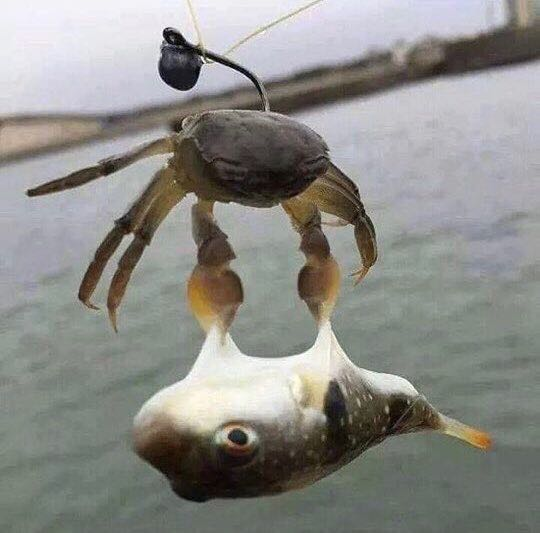
\includegraphics[clip,width=7.0cm]{./fig/kani.JPG}
  \caption{kaniの図}
  \label{fig:kani}
\end{figure}

とても愛くるしいので大好きである(二回目)


\section{おわりに}
おわりません



\begin{thebibliography}{9}
  \bibitem{kani} かに道楽,https://douraku.co.jp/ (参照日: 2019/7/2)
\end{thebibliography}

\end{document}

% ---------------------------------------------------------------

% 図を載せる
% 参照は\figref{fig:hoge}
% \begin{figure}[H]
%   \centering
%   \includegraphics[clip,width=7.0cm]{./fig/hoge.JPG}
%   \caption{hogeの図}
%   \label{fig:hoge}
% \end{figure}

% ソース載せる
% 参照は\lisref{hoge}
% \begin{lstlisting}[caption=hoge.cppのソースコード,label=hoge]
%   ソース
% \end{lstlisting}

% 表を作成する
% 参照は\tabref{tab:hoge}
% \begin{table}[H]
%   \centering
%   \begin{tabular}{c|c} \hline \hline
%     統計量 & 値 \\ \hline
%     平均 & 3167 \\ 
%     \hline
%   \end{tabular}
%   \label{tab:hoge}
% \end{table}

% 箇条書き
% \begin{itemize}
%   \item hoge
%   \item fuga
% \end{itemize}

% 数式環境
% 参照は\ref{eq:hoge}
% \begin{eqnarray}
%   \centering
%   \label{eq:hoge}
%   % 式は以下に書く
%   \sigma^2 & = & \frac{1}{N} \sum_{i=1}^{n} (x_i - m)^2
% \end{eqnarray}

% 連立方程式環境
% \begin{eqnarray}
%   \begin{cases}
%     2x + 4y = 10 & \\
%     x + 3y = 6 &
%   \end{cases}
% \end{eqnarray}
